\documentclass[a4paper]{jpconf}
% \bibliographystyle{iopart-num}
\usepackage{amsmath}
\usepackage{citesort}
\usepackage{subfigure}
\usepackage{graphicx}
\graphicspath{{fig/}}
\usepackage{ifpdf}
\ifpdf\usepackage{epstopdf}\fi
\usepackage[export]{adjustbox}

%----------------------------------------------------- 
%\usepackage{soul,ulem,color,xspace,bm}
% Suggest to remove
%\newcommand{\asrm}[1]{{\color{magenta}\sout{#1}}}
% Suggest to insert
%\newcommand{\as}[1]{\color{cyan}#1\xspace\color{black}}
% Suggest to replace
%\newcommand{\asrp}[2]{\asrm{#1} \as{#2}}
% Comment
%\newcommand{\ascm}[1]{{\color{green}\;AS: #1}}
%------------------------------------------------------

\def\apj{ApJ}
\def\mnras{MNRAS}
\def\nat{Nat}
\def\prd{Phys. Rev. D}
\def\araa{ARA\&A}                % "Ann. Rev. Astron. Astrophys."
\def\aap{A\&A}                   % "Astron. Astrophys."
\def\aaps{A\&AS}                 % "Astron. Astrophys. Suppl. Ser."
\def\aj{AJ}                      % "Astron. J."
\def\apjs{ApJS}                  % "Astrophys. J. Suppl. Ser."
\def\pasp{PASP}                  % "Publ. Astron. Soc. Pac."
\def\apjl{ApJ}                   % letter at ApJ
\def\pasj{PASJ}
\def\apss{Astroph. Space Sci.}
\def\aplett{Astroph. Lett}
\def\ssr{Space Sci. Rev.}
\def\aapr{Astron. Astroph. Reviews}
\def\physrep{Phys. Reports}
\def\memsai{Mem. Societa Astronom. Italiana}
\def\jgr{JGR}
\def\jcap{Journal of Cosmology and Astroparticle Physics}

\usepackage{xspace}
\usepackage[dvipsnames]{xcolor}
\usepackage[normalem]{ulem}
% Suggest to remove
\newcommand{\asrm}[1]{{\color{OrangeRed}\sout{#1}}}
% Suggest to insert
\newcommand{\as}[1]{\color{RoyalBlue}#1\xspace\color{black}}
% Suggest to replace
\newcommand{\asrp}[2]{\asrm{#1} \as{#2}}
% Comment
\newcommand{\ascm}[1]{{\color{ForestGreen}#1}}

\begin{document}
	\title{On electron acceleration  by mildly-relativistic shocks: PIC simulations}
	
	\author{V I Romansky$^{1}$, A M Bykov$^{1,2}$ and S M Osipov$^{1}$}
	
	\address{$^1$ Ioffe Institute, 26 Politekhnicheskaya st., St. Petersburg 194021, Russia}
	\address{$^2$ Peter the Great St. Petersburg Polytechnic University, 29 Politekhnicheskaya st., St. Petersburg 195251, Russia}
	
	\ead{romanskyvadim@gmail.com}
	
	\begin{abstract}
                 Radio observations revealed a presence of relativistic supernovae - a class of objects intermediate between the regular supernovae and gamma-ray bursts. The typical Lorentz-factors of plasma flows in relativistic radio-bright supernovae were estimated to be about $1.5$. Mildly relativistic shocks in electron-ion plasmas are known to efficiently accelerate radio-emitting electrons if the shock is subluminous. The inclination angle of the velocity of subluminous shock to the ambient magnetic field should be below a critical angle which depends on the Mach number and the plasma magnetization parameter.  In this paper we present particle-in-cell modeling of electron acceleration by mildly-relativistic collisionless shock of different obliquity in a plasma with ratio of the magnetic energy to the bulk kinetic energy $\sigma \approx 0.004$ which is of interest for the relativistic supernovae modeling. It was shown earlier that  a development of the ion scale Bell-type instability in electron-ion relativistic shock may have a strong influence on the electron injection and acceleration. In the time period of about $1500 \omega_{pi}^{-1}$  ($\omega_{pi}$ is the ion plasma frequency) after the shock initialization the  magnetic field fluctuations  generated by Bell's instability may significantly decreases number of accelerated electrons even in a sub-luminous shock. We study here the evolution of the electron spectra of subluminous shocks of different obliquity. This is important to for modeling of synchrothron spectra from relativistic supernovae.
	\end{abstract}
	
	\section{Introduction}
	Relativistic shocks are playing an important role  in modeling of luminous high energy objects in  astrophysics. They can be generated in the supernovae \cite{2010Natur.463..513S,2007ApJ...667..351W}, the accreting supermassive black holes \cite{1984RvMP...56..255B}, the stellar masses black holes \cite{2019MmSAI..90...57M,1999PhR...314..575P,2014LNP...876.....R} and pulsar wind nebulae \cite{Amato2006,2017SSRv..207..235B,2017JPlPh..83e6301K,2019ApJ...876L...8B}. Relativistic shocks in astrophysical objects are sources of cosmic rays \cite{2012SSRv..173..309B,2015SSRv..191..519S,Pelletier2017} and can accelerate particles to ultra-high energies \cite{Wang2007,2009JCAP...11..009L,BEMO18}. 
	
	The presence of high energy non-thermal particles leads to development of various magneto-hydrodynamic instabilities (see e.g. \cite{MD2001,Amato09,Bykov2013}). Bell's instability \cite{Bell04} can be the most significant due to it's large growth rate. Instabilities may modify the flow and has strong influence on the process of particle acceleration \cite{Crumley2019,2021MNRAS.501.4837L,2021MNRAS.502.5065L}. Namely, it was realized that Bell's instability is producing the strong ion-scale magnetic fluctuations which 
	provide on the electron scales some macroscopic size regions of the superluminal shock obliquity which locally suppress the electron injection. The shock rippling effect is important for the electron spectra formation in the mildly-relativistic shocks.
	In the simulations \cite{Crumley2019} the electron spectra evolution was demonstrated in a mildly-relativistic shock   of an inclination angle 10 degrees. The magnetic fluctuations produced by the Weibel instability initially efficiently reflect and energize both ions and electrons. After the time period of about $1500 \omega_{pi}^{-1}$  the efficiency of electron acceleration by the shock drops down significantly because of developing of Bell's instability which increases the transversal magnetic field. The proton spectrum in this simulations was not strongly affected in the Bell-mediated shock.   Given the significant interest of non-thermal particle acceleration by the subluminal mildly-relativistic shocks we present below results of particle-in-cell modeling of electron and proton acceleration by the mildly-relativistic shocks of different inclination angles. 
	
	
	\section{Numerical setup}
	In this work we use particle-in-cell code Smilei \cite{Smilei18} for modeling mildly-relativistic collisionless shocks. We initialize two-dimensional space domain, with electron-proton plasma flowing into simulation box through the right boundary and reflecting wall on the left boundary. In the transversal direction boundary conditions are periodic.
	
	The simulation parameters are : the initial flow Lorentz factor $\Gamma = 1.5$, the flow magnetization $\sigma = \frac{B^2}{4\pi\Gamma (n_p m_p + n_e m_e) c^2} = 0.004$. The dimensionless thermal energy $\Delta \gamma = \frac{k T}{m_p c^2}$ is equal to $10^{-4}$ and the electron mass is increased up to $m_e = \frac{m_p}{100}$. The size of the simulation box along the $x$ axis is $L_x = 30000\frac{c}{\omega_p}$ and in the transverse direction $L_y = 200\frac{c}{\omega_p}$, where $\omega_p = \sqrt{\frac{4\pi q^2 n}{\Gamma m_e}}$ is the plasma frequency. These scales correspond to $150000$ and $1000$ grid points in $x$ and $y$ directions, respectively. 
	
	Inclination angle of magnetic field due to shock velocity varies in different setups from $\theta = 20^\circ$ to $\theta = 40^\circ$. These values are chosen to contain critical angle, which is defined by the equation $c\cdot \cos(\theta_{crit})=v_{shock}$, where all values are measured in the upstream rest frame, and is equal approximately $30$ degrees. If inclination angle is larger then critical value, shock becomes superluminal - particle can not escape from it to upstream, even moving along the field lines with speed of light \cite{Pelletier2017,Sironi2011}. The maximum efficiency of particle acceleration is near the critical angle, and is less below this angle \cite{Romansky18}. Magnetic field is lying in the simulation plane.
	
	
	\section{Results}
	
	Profiles of transversal magnetic field, obtained from numerical simulation, show significant field amplification in precursor of shock wave, see figure \ref{field}. It is result of development of instabilities in plasma, particularly Bell's instability \cite{Bell04}, which growth rate is larger than growth rate of other instabilities.
	
	\begin{figure}[h!]
		\centering
		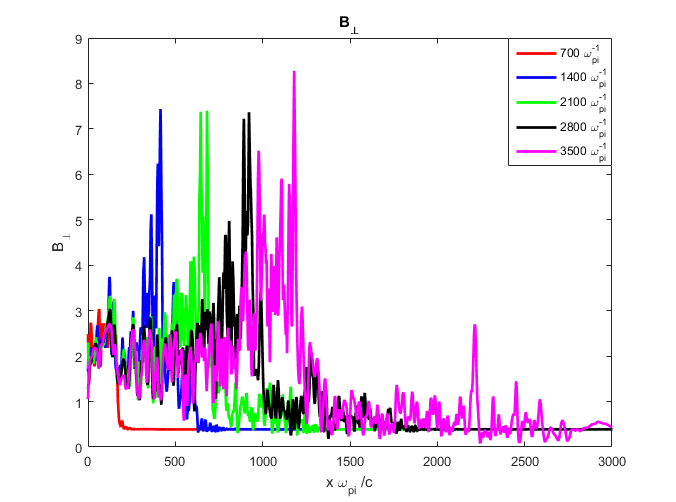
\includegraphics[width=0.50\textwidth]{fig/Bnorm.png} 
		\caption{Temporal evolution of the transversal magnetic field.}
		\label{field}
	\end{figure}
	
	It is known, that development of Bell's instability can suppress electron acceleration \cite{Crumley2019,2021MNRAS.501.4837L,2021MNRAS.502.5065L}. We study this phenomena with different inclination angles of magnetic field. Spectrum of electrons is shown in figure \ref{spectrume}. One can see, that electron acceleration has strong dependence on inclination angle, and when it is more than critical value (at $\theta = 40^\circ$), non-thermal component almost disappears. For smaller angles electron distribution function at high energies $(\Gamma > 300)$ depends on time, and it maximizes at times about 1400 inverse proton plasma frequencies for angles $\theta=20^\circ, \theta=30^\circ$, and 2100 and inverse proton plasma frequencies for $\theta = 33^\circ$. After reaching the maximum value the electron distribution magnitude starts decreasing at high energies. It may by explained as consequence of magnetic field amplification. Instabilities increase the transverse magnetic field and also the angle between field and shock velocity. As a result shock becomes quasi-perpendicular and can not effectively accelerate particles \cite{Sironi2011,Romansky18}. On the other hand, proton distribution function constantly increases in time for sub-critical angles, and almost does not have non-thermal component for $\theta = 40^\circ$, as shown in figure \ref{spectrump}. We assume, that oscillating transverse field has the strongest influence on the smallest scales, and suppresses the electrons injection into acceleration process, while protons still can be accelerated. Also, one can see, that temporal evolutions of electron and proton spectrums are correlated. In case of inclination angle $\theta = 33^\circ$ proton distribution function grows slower then for smaller angles. And electron distribution in this case is maximizes at larger time. This correlation confirms the assumption, that instability suppressing electron acceleration is caused by accelerated protons.
	
	
	\begin{figure}[h!]
		\centering
		\begin{minipage}{0.48\textwidth}
			\centering
			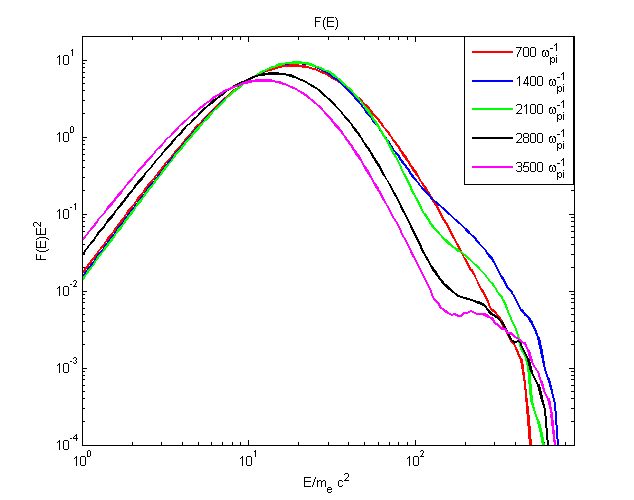
\includegraphics[width=0.98\textwidth]{fig/spectrum20.png} 
		\end{minipage}\hfill
		\begin{minipage}{0.48\textwidth}
			\centering
			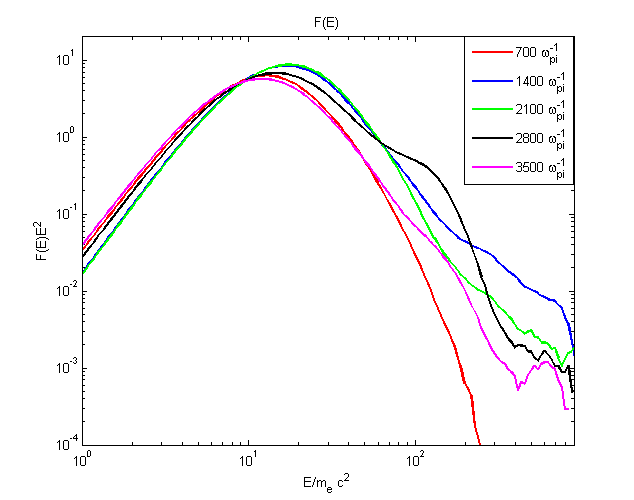
\includegraphics[width=0.98\textwidth]{fig/spectrum30.png} 
		\end{minipage}
		\begin{minipage}{0.48\textwidth}
			\centering
			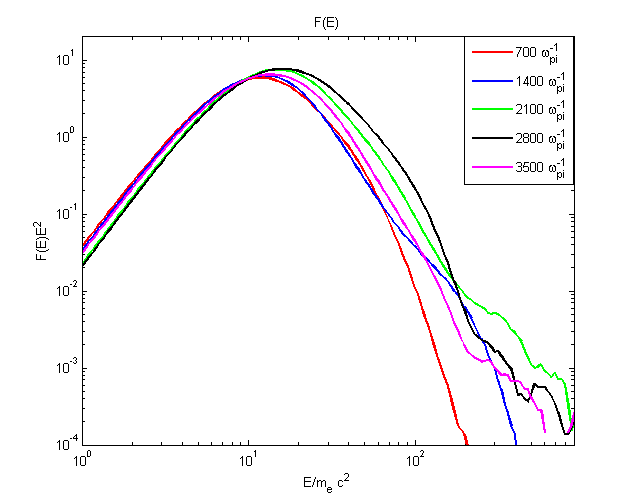
\includegraphics[width=0.98\textwidth]{fig/spectrum33.png} 
		\end{minipage}
		\begin{minipage}{0.48\textwidth}
			\centering
			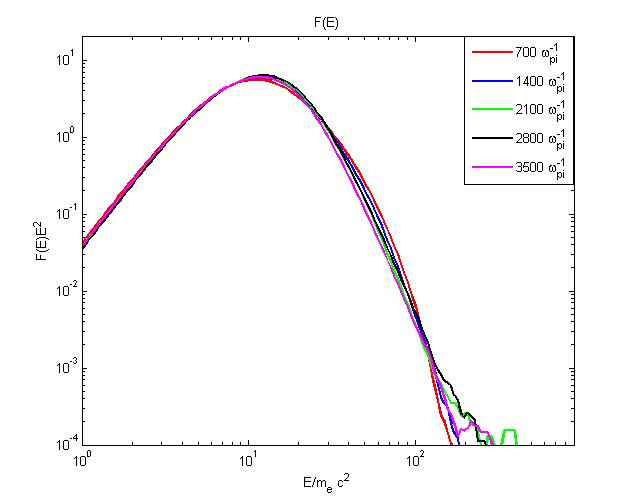
\includegraphics[width=0.98\textwidth]{fig/spectrum40.png} 
		\end{minipage}
		\caption{Temporal evolution of electron spectrum in shocks with different magnetic field inclination angles. Top row: left $\theta = 20^\circ$, right $\theta = 30^\circ$, bottom row: left $\theta = 33^\circ$, right $\theta = 40^\circ$}
		\label{spectrume}
	\end{figure}

\begin{figure}[h!]
	\centering
	\begin{minipage}{0.48\textwidth}
		\centering
		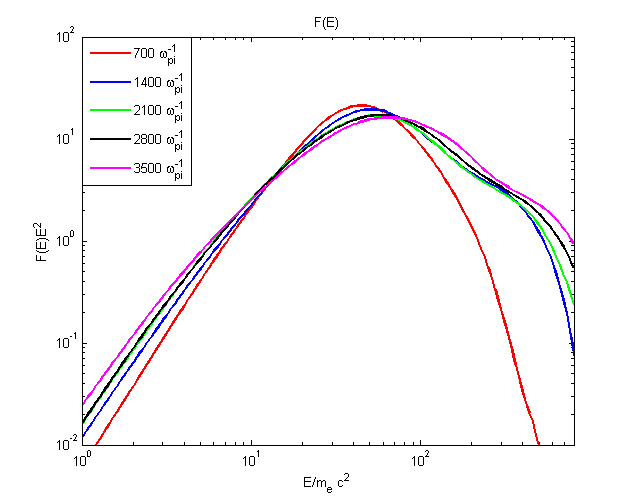
\includegraphics[width=0.98\textwidth]{fig/spectrump20.png} 
	\end{minipage}\hfill
	\begin{minipage}{0.48\textwidth}
		\centering
		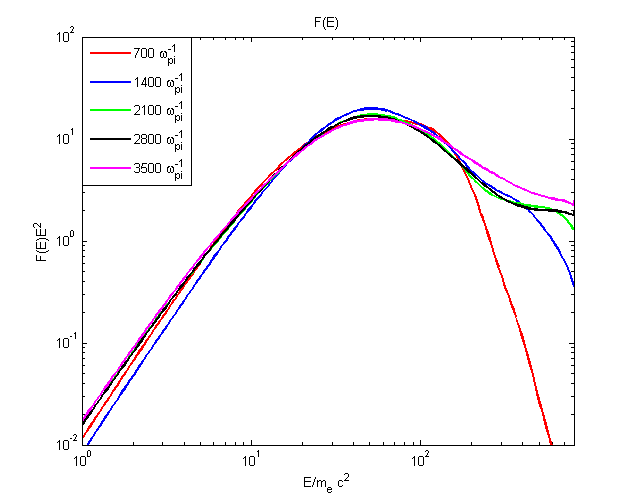
\includegraphics[width=0.98\textwidth]{fig/spectrump30.png} 
	\end{minipage}
	\begin{minipage}{0.48\textwidth}
		\centering
		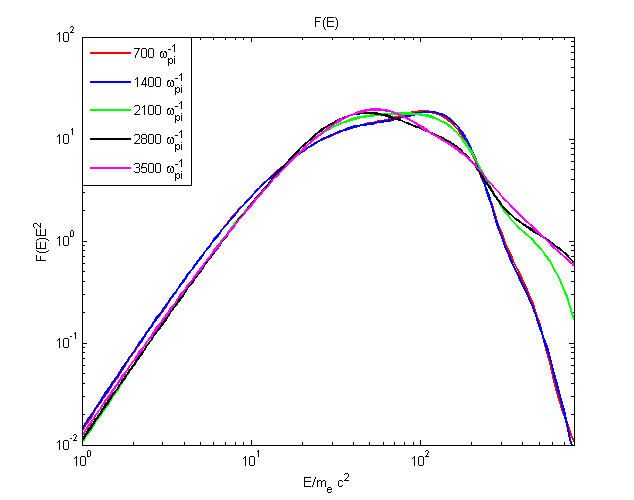
\includegraphics[width=0.98\textwidth]{fig/spectrump33.png} 
	\end{minipage}
	\begin{minipage}{0.48\textwidth}
		\centering
		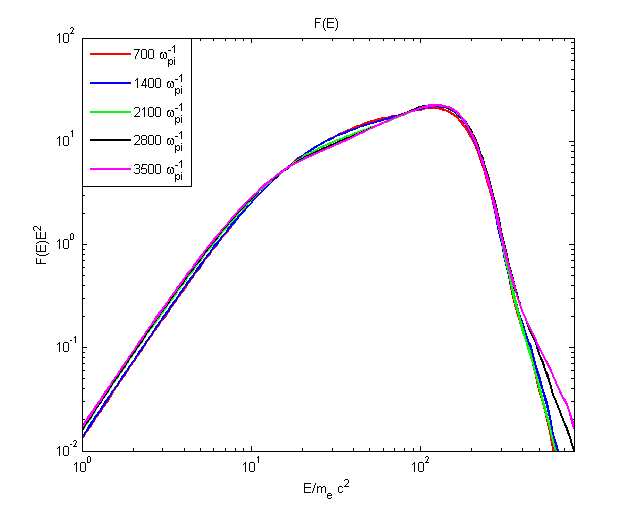
\includegraphics[width=0.98\textwidth]{fig/spectrump40.png} 
	\end{minipage}
	\caption{Temporal evolution of proton spectrum in shocks with different magnetic field inclination angles. Top row: left $\theta = 20^\circ$, right $\theta = 30^\circ$, bottom row: left $\theta = 33^\circ$, right $\theta = 40^\circ$}
	\label{spectrump}
\end{figure}
	

	
	\section{Conclusions}
	
	Details of electron acceleration are important for correct interpretations of observations of the  synchrothron radiation from astrophysical sources. Particle-in-cell simulation has been used to demonstrate magnetic instabilities influence on electron acceleration in mildly-relativistic electron-ion shock. It is shown, that amplification of magnetic field suppresses formation of electron spectrum at high energies while proton spectrum can grow monotonously in time in subluminal shock. Also, we demonstrated that groth of proton spectrum is correlated with decreasing of electron acceleration, and resulting  electron spectrum strongly depends on magnetic field inclination angle. This effect should be taken into account for deriving parameters of source of synchrothron radiation via analysis of spectrum. Further particle-in-cell simulations with a wider spatial and energetical ranges will allow to study the influence of instabilities on electron spectrum more precisely.
	
	
	\ack
	The authors were supported by RSF grant 21-72-20020.
	Some results of the work were obtained using computational resources of Peter the Great Saint-Petersburg Polytechnic University Supercomputing Center (http://scc.spbstu.ru)
	
	\section*{References}
	% \bibliographystyle{apalike}
	\bibliographystyle{iopart-num}

	\bibliography{bibliogr}
\end{document}